\documentclass[12pt]{report}
\usepackage[T2A]{fontenc}
\usepackage[utf8]{inputenc}
\usepackage[english,russian]{babel}
\usepackage{listings}
\usepackage{graphicx}

\usepackage{tikz}
\usepackage{pgfplots}
\pgfplotsset{compat=1.9}

\renewcommand\contentsname{Оглавление}

\usepackage{geometry}
\geometry{left=2cm}
\geometry{right=1.5cm}
\geometry{top=1cm}
\geometry{bottom=2cm}

% Для листинга кода:
\lstset{ %
language=python,                 % выбор языка для подсветки (здесь это С)
basicstyle=\small\sffamily, % размер и начертание шрифта для подсветки кода
numbers=left,               % где поставить нумерацию строк (слева\справа)
numberstyle=\tiny,           % размер шрифта для номеров строк
stepnumber=1,                   % размер шага между двумя номерами строк
numbersep=5pt,                % как далеко отстоят номера строк от подсвечиваемого кода
showspaces=false,            % показывать или нет пробелы специальными отступами
showstringspaces=false,      % показывать или нет пробелы в строках
showtabs=false,             % показывать или нет табуляцию в строках
frame=single,              % рисовать рамку вокруг кода
tabsize=2,                 % размер табуляции по умолчанию равен 2 пробелам
captionpos=t,              % позиция заголовка вверху [t] или внизу [b] 
breaklines=true,           % автоматически переносить строки (да\нет)
breakatwhitespace=false, % переносить строки только если есть пробел
escapeinside={\#*}{*)}   % если нужно добавить комментарии в коде
}

\usepackage{titlesec} % подключаем нужные пакеты
\newcommand{\hsp}{\hspace{20pt}} % длина линии в 20pt
\titleformat{\chapter}[hang]{\Huge\bfseries}{\thechapter{.}\hsp}{0pt}{\Huge\bfseries}

\begin{document}

    \begin{titlepage}

        \begin{center}
            \large
            {\sl Государственное образовательное учреждение высшего профессионального образования\\
            {\bf«Московский государственный технический университет имени Н. Э. Баумана»\\
				(МГТУ им. Н.Э. Баумана)}}
				\noindent\rule{\textwidth}{2pt}
		\end{center}
				{\large ФАКУЛЬТЕТ\hsp«Информатика и система управления»}\\
				{\large КАФЕДРА\hsp«Программное обеспечение ЭВМ и информационные технологии»}\\
		\begin{center}
            \vspace{3cm}

				{\scshape\large Лабораторная работа №1 \par}
				\vspace{0.5cm}	
				{\scshape\large по курсу «Анализ алгоритмов» \par}
				\vspace{1.5cm}
				{\huge\bfseries Расстояние Левенштейна и Дамерау-Левенштейна \par}
				\vspace{2cm}
				\large Выполнил: Сорокин А.П., гр. ИУ7-52Б\\
				\vspace{0.5cm}
				{\large Преподаватели: Волкова Л.Л., Строганов Ю.В.}
			
				\vfill
				\large \textit {Москва, 2019г.}
            
            \end{center}

    \end{titlepage}
	
	\tableofcontents

	\chapter*{Введение}
	\addcontentsline{toc}{chapter}{Введение}

	{\bf Расстояние Левенштейна} определяет минимальное количество операций, необходимых для превращения одной строки в другую. Задача определения такого минимума актуальна, так как она решает множество проблем в теории информации и компьютерной лингвистике, например:

	\begin{itemize}
		\item исправление ошибок в словах при вводе (при в поисковых ситсемах, базах данных, программах автоматического определения текста);
		\item сравнении текстовых файлов (к примеру, утилита diff);
		\item сравнение белков, генов и хромосом в биоинформатике.
	\end{itemize}

    \chapter{Аналитическая часть}

	 \section{Задачи}
	Цель лабораторной работы: исследовать расстояния Левенштейна и Дамерау-Левенштейна. Для достижения этой цели были поставлены следующие задачи: 
	\begin{itemize}
		\item изучить алгоритмы вычисления расстояний между строками;
		\item применить методы динамического программирования для матричной реализации алгоритмов;
		\item сравнить матричную и рекурсивную реализацию алгоритмов;
		\item оценить эффективность каждой из реализаций по времени и памяти.
	\end{itemize}

	 \section{Описание алгоритмов}
    При нахождении расстояния Левенштейна определяется минимального количество операций следующих видов:
	\begin{itemize}
		\item вставка (I - insert);
		\item удаление (D - delete);
		\item замена (R - replace);
		\item совпадение (M - match).	
	\end{itemize}
	При нахождении расстояния Дамерау-Левенштейна добавляется операция транспозиции (T - transpose), или перестановки двух соседних символов.\\

	Таким образом, если заданы две строки $S_{1}$ и $S_{2}$ с длинами $m$ и $n$ соответственно над некоторым алфавитом, то расстояние Левенштейна можно вычислить по следующей рекуррентной формуле:

	\begin{equation}
	D(S_{1}[1..m], S_{2}[1..n]) = min(D(S_{1}[1..m-1], S_{2}[1..n] + 1),\\
	\end{equation}
	\begin{equation}
	D(S_{1}[1..m], S_{2}[1..n-1]+1),\\
	\end{equation}
	\begin{equation}
	D(S_{1}[1..m-1], S_{2}[1..n-1]+m(S_{1}[m], S_{2}[n])))
	\end{equation}
	где
	\begin{displaymath}
	m(a,b) = \left\{
	\begin{array}{ll}
		0, a=b\\
		1, a \neq b
	\end{array} \right.,
	\end{displaymath}\ \\
	Соотношения в рекурретной формуле отвечают за соотвествующие разрешённые операции:
	\begin{itemize}
		\item (1.1) - вставка;
		\item (1.2) - удаление;
		\item (1.3) - замена или совпадение в зависимости от результата $m(a,b)$.	
	\end{itemize}

	При вычислении расстояния Дамерау-Левенштейна в рекурретную формулу вносится дополнительное соотношение в минимум:
	\begin{equation}
	\label{damerau}
	D(S_{1}[1..m-2], S_{2}[1..n-2])+1
	\end{equation}
Соотношение ~(\ref{damerau}) вносится в качестве дополнительного аргумента минимума только при выполнении следующих условий:
	\begin{itemize}
		\item $m > 2,n > 2$;
		\item $S_{1}[m] = S_{2}[n-1]$;
		\item $S_{1}[m-1] = S_{2}[n]$.	
	\end{itemize}

	Тривиальным случаем в рекуррентной формуле является случай, когда одна из строк пустая. В этом случае расстояние Левенштейна равно длине другой строки.

	Расстояния Левенштейна и Дамерау-Левенштейна можно также вычислить, используя матрицу, в которое разрешённые операции определены следующим образом:
	\begin{itemize}
		\item движение по столбцам вправо - вставка;
		\item движение по строкам вверх - удаление;
		\item движение по диагонали - замена/совпадение.
	\end{itemize}

	\chapter{Конструкторская часть}

	\section{Схемы алгоритмов}
	\begin{figure}
		\centering
		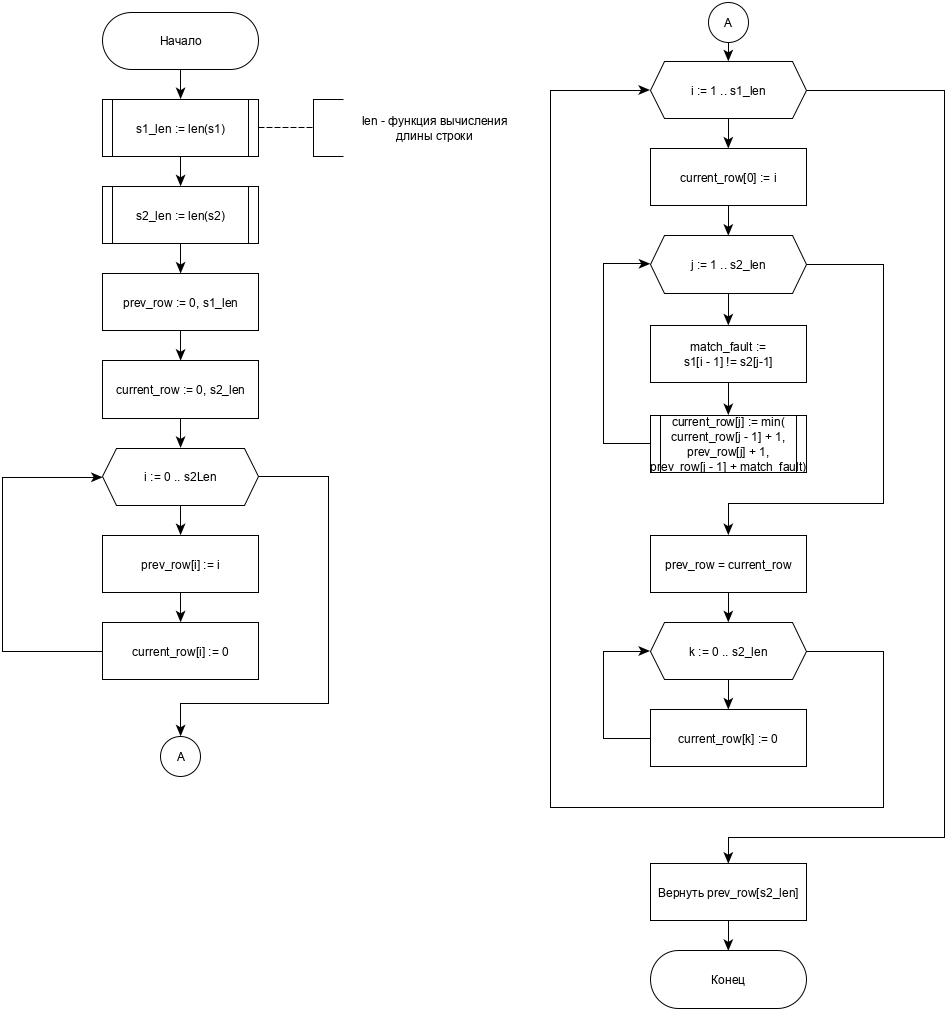
\includegraphics[width=1\linewidth]{leven}
		\caption{Алгоритм Левенштейна}
		\label{fig:leven}
	\end{figure}

	\begin{figure}
		\centering
		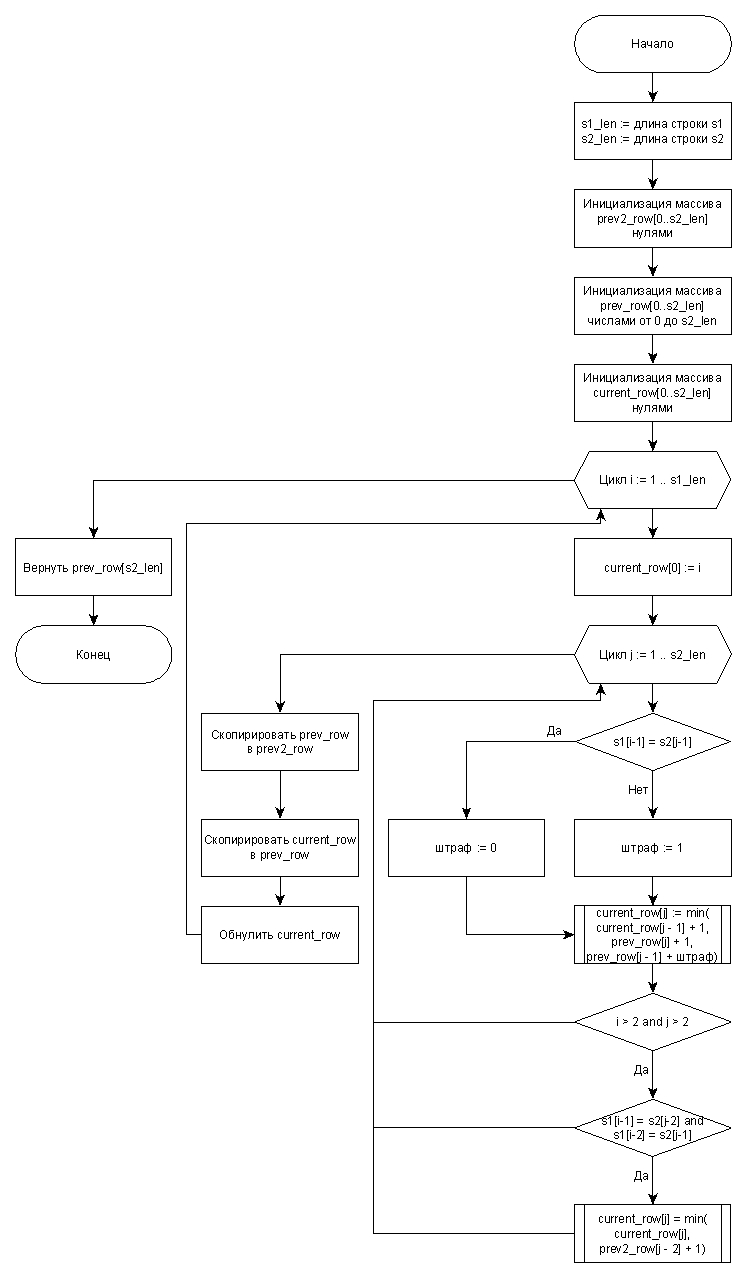
\includegraphics[width=1\linewidth]{damleven}
		\caption{Алгоритм Дамерау-Левенштейна (матричная реализация)}
		\label{fig:damleven}
	\end{figure}
	
	\begin{figure}
		\centering
		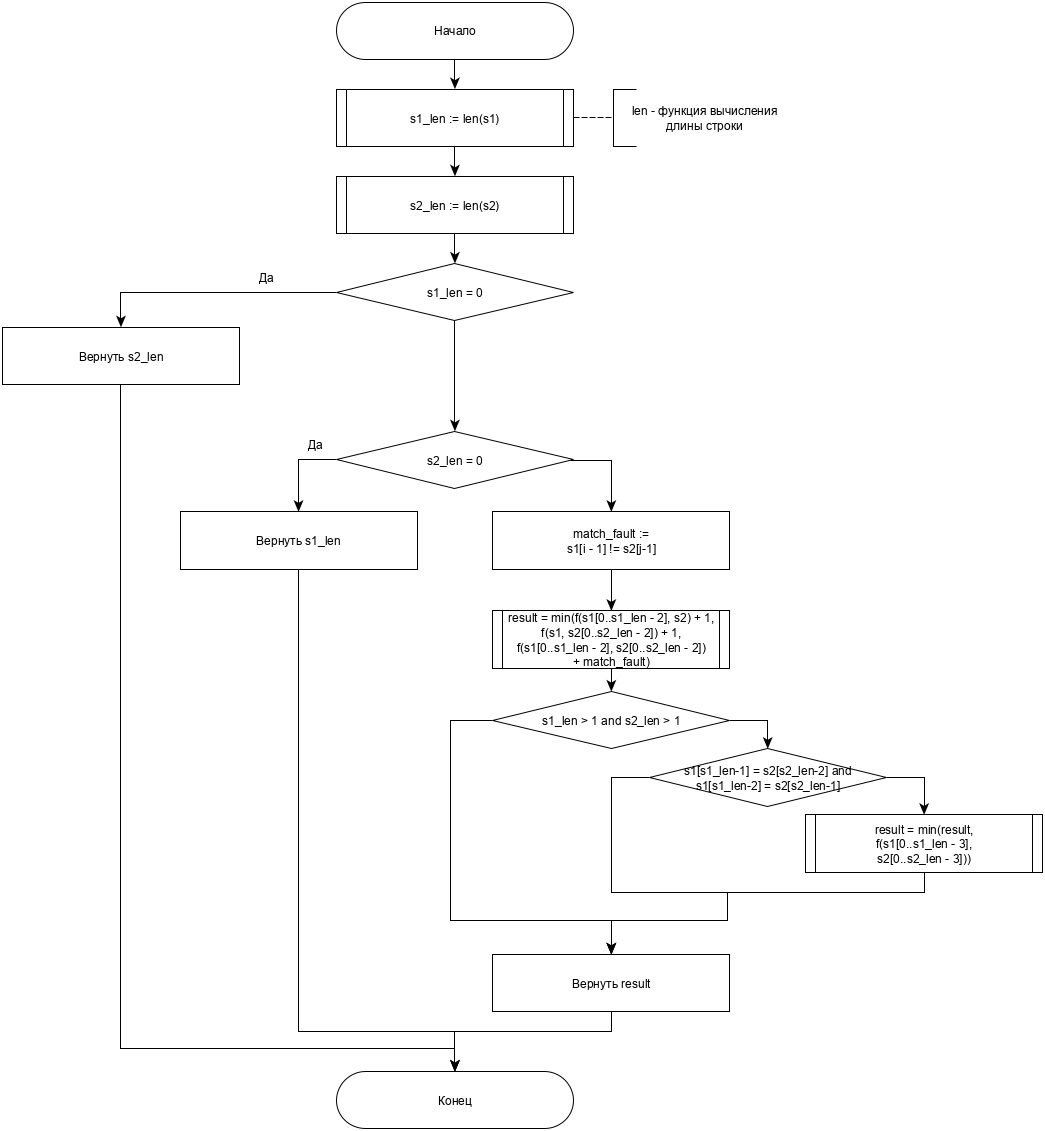
\includegraphics[width=1\linewidth]{damleven_r}
		\caption{Алгоритм Дамерау-Левенштейна (рекурсивная реализация)}
		\label{fig:damlevenr}
	\end{figure}
	
	

	\section{Структуры данных}
	
	\chapter{Технологическая часть}
	\section{Требования к программному обеспечению}
	\section{Средства реализации}
   \section{Листинг кода}
	\begin{lstlisting}[label=some-code,caption=Расстояние Левенштейна (матрично)]
	def str_distance(s1, s2, to_print=False):
	    s1_len = len(s1)
	    s2_len = len(s2)
	
	    # initialization of first two rows
	    prev_row = [i for i in range(s2_len + 1)]   # first row - [0, 1, ..., n]
	    current_row = [0] * (s2_len + 1)
	
	    if to_print:
	        print(prev_row)
	
	    for i in range(1, s1_len + 1):          # row loop
	        # current row fill
	        current_row[0] = i
	        for j in range(1, s2_len + 1):                  # column loop
	            match_fault = int(s1[i - 1] != s2[j - 1])            # symbol match
	            current_row[j] = min(current_row[j - 1] + 1,         # horizontal
	                                 prev_row[j] + 1,                # vertical
	                                 prev_row[j - 1] + match_fault)  # diagonal
	
	        if to_print:
	            print(current_row)
	
	        # row switching
	        prev_row = current_row
	        current_row = [0] * (s2_len + 1)
	
	    return prev_row[-1]     # value in bottom right corner of table
	\end{lstlisting}

	\begin{lstlisting}[label=some-code,caption=Расстояние Дамерау-Левенштейна (матрично)]
	def str_distance(s1, s2, to_print=False):
    s1_len = len(s1)
    s2_len = len(s2)

    # initialization of first two rows
    prev2_row = [0] * (s2_len + 1)
    prev_row = [i for i in range(s2_len + 1)]
    current_row = [0] * (s2_len + 1)

    if to_print:
        print(prev_row)

    for i in range(1, s1_len + 1):          # row loop
        # current row fill
        current_row[0] = i
        for j in range(1, s2_len + 1):                  # column loop
            match_fault = int(s1[i - 1] != s2[j - 1])      # if symbol matches
            current_row[j] = min(current_row[j - 1] + 1,         # horizontal
                                 prev_row[j] + 1,                # vertical
                                 prev_row[j - 1] + match_fault)  # diagonal

            # transposition check
            if i > 2 and j > 2:
                if s1[i - 1] == s2[j - 2] and s1[i - 2] == s2[j - 1]:
                    current_row[j] = min(current_row[j],
                                         prev2_row[j - 2] + 1)

        if to_print:
            print(current_row)

        # row switching
        prev2_row = prev_row
        prev_row = current_row
        current_row = [0] * (s2_len + 1)

    return prev_row[-1]         # value in bottom right corner of table
	\end{lstlisting}

	\begin{lstlisting}[label=some-code,caption=Расстояние Дамерау-Левенштейна (рекурсивно)]
		def str_distance(s1, s2):
	    s1_len = len(s1)
	    s2_len = len(s2)
	
	    if s1_len == 0:
	        return s2_len
	    if s2_len == 0:
	        return s1_len
	
	    match_fault = int(s1[-1] != s2[-1])
	
	    result = min(str_distance(s1[:-1], s2) + 1,
	                 str_distance(s1, s2[:-1]) + 1,
	                 str_distance(s1[:-1], s2[:-1]) + match_fault)
	
	    if s1_len > 1 and s2_len > 1:
	        if s1[-1] == s2[-2] and s1[-2] == s2[-1]:
	            result = min(result, str_distance(s1[:-2], s2[:-2]) + 1)
	
	    return result
	\end{lstlisting}

	\newpage

	\section{Тесты}
	Для проверки корректности работы были подготовлены следующие функциональные тесты:\\
	\begin{table}
		\begin{tabular}{|c|c|c|c|}
		\hline
		\bf{Строка 1} & \bf{Строка 2} & \bf{Ожидание} & \bf{Результат}\\\hline
		<пустая> & <пустая> & 0 0 0 & 0 0 0\\\hline
		<пустая> & а & 1 1 1 & 1 1 1\\\hline
		а & <пустая> & 1 1 1 & 1 1 1\\\hline
		а & а & 0 0 0 & 0 0 0\\\hline
		а & б & 1 1 1 & 1 1 1\\\hline
		азы & базы & 1 1 1 & 1 1 1\\\hline
		компютер & компьютер & 1 1 1 & 1 1 1\\\hline
		данны & данные & 1 1 1 & 1 1 1\\\hline
		email.ru & mail.ru & 1 1 1 & 1 1 1\\\hline
		programmmer & programmer & 1 1 1 & 1 1 1\\\hline
		mail.rus & mail.ru & 1 1 1 & 1 1 1\\\hline
		ашибка & ошибка & 1 1 1 & 1 1 1\\\hline
		алгоритм & алгорифм & 1 1 1 & 1 1 1\\\hline
		копия & копии & 1 1 1 & 1 1 1\\\hline
		укрсовой & курсовой & 2 1 1 & 2 1 1\\\hline
		аглоритм & алгоритм & 2 1 1 & 2 1 1\\\hline
		унивре & универ & 2 1 1 & 2 1 1\\\hline
		курс & курсовой & 4 4 4 & 4 4 4\\\hline
		курсовой & курс & 4 4 4 & 4 4 4\\\hline
		курсовой & курсовик & 2 2 2 & 2 2 2\\\hline
		код & закодировать & 9 9 9 & 9 9 9\\\hline
		закодировать & код & 9 9 9 & 9 9 9\\\hline
		ccoders & recoding & 5 5 5 & 5 5 5\\\hline
		header & subheader & 3 3 3 & 3 3 3\\\hline
		subheader & header & 3 3 3 & 3 3 3\\\hline
		subheader & overheader & 4 4 4 & 4 4 4\\\hline
		\end{tabular}
		\caption{Функциональные тесты}
	\end{table}

	\chapter{Экспериментальная часть}
	\section{Примеры работы}
	
   \section{Исследование времени выполнения}
   \begin{tikzpicture}
   \begin{axis}
   \addplot coordinates {
   	(1,2) (2,5) (3,9) (4,14) (5,1940) (6,3180) (7,38700) (8,51200) (9,64100) (10,71299) 
   };
	\addplot coordinates {
		(1,2) (2,5) (3,9) (4,15) (5,2109) (6,6709) (7,42300) (8,55600) (9,69299) (10,78000) 
	};
   \end{axis}
   \end{tikzpicture}
   
   \begin{tikzpicture}
   \begin{axis}
   \addplot coordinates {
   (1,2) (2,5) (3,9) (4,15) (5,2109) (6,6709) (7,42300) (8,55600) (9,69299) (10,78000) 
   };
   \addplot coordinates {
   	(1,2) (2,9) (3,45) (4,233) (5,119869) (6,667230) (7,37966999) (8,212703900) (9,1137897600) (10,6538969300) 
   };
   \end{axis}
   \end{tikzpicture}

   \chapter*{Заключение}
	\addcontentsline{toc}{chapter}{Заключение}
	Алгоритмы нахождения расстояния Левенштейна и Дамерау-Левенштейна между строками были изучены и реализованы: были реализованы три варианта алгоритма для получения навыка динамического программирования.\\
	Были исследованы затраты данных вариантов реализации по времени и памяти. Экспериментально было подтверждено, что рекурсивный вариант реализации алгоритма значительно проигрывает матричным вариантам при росте длины входных строк по обоим показателям.

	\chapter*{Список литературы}
	\addcontentsline{toc}{chapter}{Список литературы}

\end{document}
